\chapter{O agora}\label{cap:agora}

O capítulo anterior mediu o corte no espaço: onde a série começa e termina. Este mede o corte no
\textbf{tempo}. Há um instante em que a decisão é tomada, e os dados em que ela se apoia são de antes
disso; a distância entre os dois é o atraso, e quase ninguém o declara.

\section{O dado que chega velho}

O atraso entra no corte de um jeito simples: a barreira que vale hoje é a que
foi calculada com o dado de \emph{d} dias atrás, sobre a janela de \numAgoraJanela{} dias. Com \emph{d} zero isso é exatamente o corte, e a identidade vale por construção --- o atraso não muda o instrumento, muda a idade do dado que ele lê.

Medida no índice, nos \numEntregaDias{} dias em que havia janela suficiente dentro dos \numAgoraDias{}
pregões da série --- um dia menos para cada dia de atraso ---, a entrega do corte é esta.

\begin{table}[htbp]
  \centering
  \small
  \begin{tabular}{rrr}
    \hline
    atraso do & entrega & em razão da \\
    dado (dias) & medida & conta do corte \\
    \hline
    nenhum & \numAgoraEntregaZero & \numAgoraRazaoZero \\
    um & \numAgoraEntregaUm & \numAgoraRazaoUm \\
    cinco & \numAgoraEntregaCinco & \numAgoraRazaoCinco \\
    vinte e um & \numAgoraEntregaVinteEUm & \numAgoraRazaoVinteEUm \\
    sessenta e três & \numAgoraEntregaSessentaETres & \numAgoraRazaoSessentaETres \\
    duzentos e cinquenta e dois & \numAgoraEntregaDuzentosECinquentaEDois & \numAgoraRazaoDuzentosECinquentaEDois \\
    \hline
  \end{tabular}
  \caption{A entrega do corte contra a idade do dado, no índice. A conta do corte é de
    \numAgoraPromessa{}, e é ela que a última coluna toma por referência.}
  \label{tab:atraso-do-dado}
\end{table}

Um dia de atraso não se nota. Um ano de atraso entrega \numAgoraRazaoDuzentosECinquentaEDois{} vezes a conta do
corte: o instrumento passa a romper \numAgoraEntregaDuzentosECinquentaEDois{} dos dias onde a conta
pede \numAgoraPromessa{}. E o atraso, na prática, nunca é zero: o dado fecha depois do dia que
descreve, e o intervalo entre o fechamento e a decisão é uma escolha de quem opera.

\section{O atraso não custa dias}

A tentação é ler a tabela acima como um preço por dia de atraso. Não é, e o motivo é aritmético.

\begin{proposicao}[o atraso não cobra dias]\label{prop:atraso-parado}
Num mundo cuja lei não muda no tempo e cujos dias são trocáveis, a entrega do corte não depende do
atraso: para qualquer $d$, a chance de o dia de hoje romper uma barreira erguida sobre os $n$ dias
que terminam $d$ dias antes é a mesma.
\end{proposicao}

\begin{proof}
A barreira de hoje é o $k$-ésimo pior daqueles $n$ dias, e o dia julgado é o de hoje, de modo que
a pergunta é sobre o posto de um dia entre $n+1$. Sob permutabilidade os $n+1$ dias são trocáveis,
o posto do dia de hoje é uniforme entre eles, e a chance de ele estar entre os $k$ piores é
$k/(n+1)$ --- a \cref{prop:conta}, para todo $d$. O atraso desloca a janela no tempo, e a troca de
$d$ não muda a lei de nenhum dos $n+1$ dias.
\end{proof}

É o que a medição do controle encontra. No mesmo experimento em \numAgoraSementes{} mundos que
\textbf{não} mudam, a entrega do corte com atraso de nenhum dia a \numAgoraAtrasoMaior{} dias fica
entre \numAgoraParadoMenor{} e \numAgoraParadoMaior{} --- uma variação de \numAgoraParadoVariacao{}
entre o atraso nenhum e o de um ano, que é o tamanho do ruído contra a proposição. O atraso de um
ano move a taxa no quarto decimal: \numAgoraParadoZero{} no atraso nenhum,
\numAgoraParadoVinteEUm{} em vinte e um dias e \numAgoraParadoMaior{} com um ano.

O que a proposição supõe é o que o mundo que muda quebra, e ali a barreira de ontem já mede outra
coisa. \textbf{O atraso não cobra dias; ele cobra a mudança que coube dentro dele.}

\section{O que ele cobra, então}

Para ver a cobrança é preciso olhar onde o mundo muda. O mundo que muda dobra de uma vez no meio
da série, e a leitura é feita só na janela que segue a mudança --- os \numAgoraHorizonte{} dias
seguintes.

\begin{figure}[htbp]
  \centering
  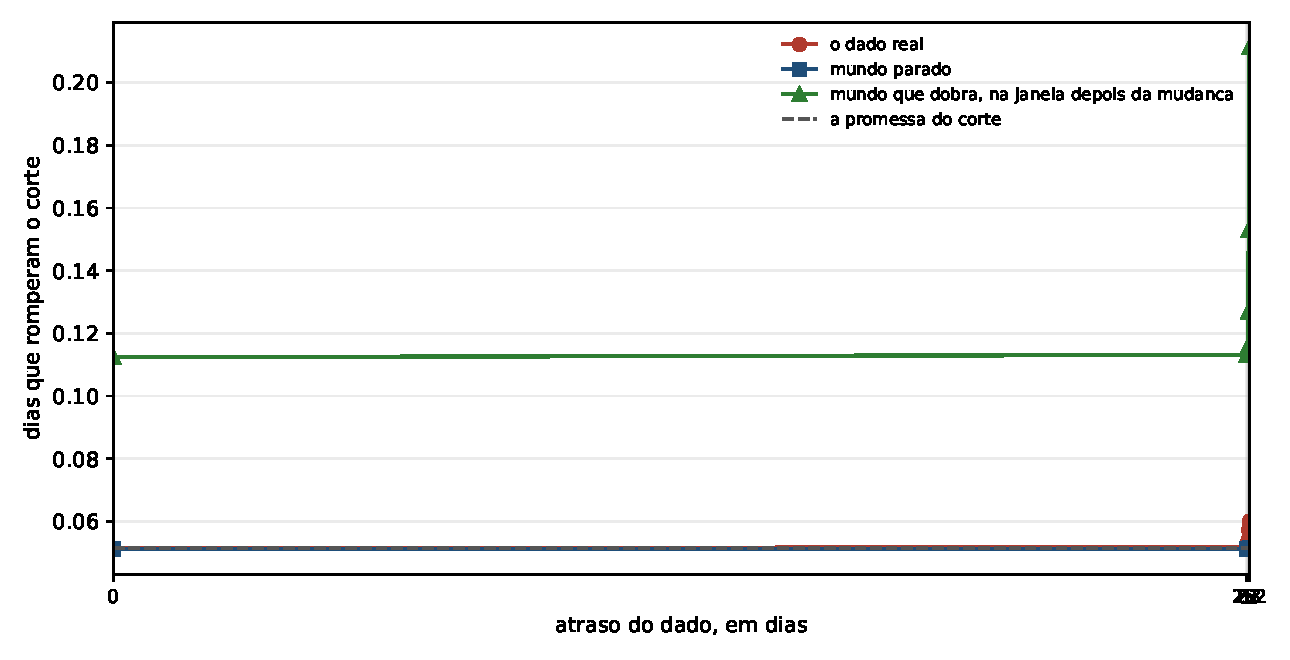
\includegraphics[width=\linewidth]{figuras/E19_o_agora_1.pdf}
  \caption{A entrega do corte contra a idade do dado, nas três situações: o dado real, o mundo que
    não muda e a janela que segue uma mudança. As duas de baixo ficam em cima da promessa em
    qualquer atraso; a de cima é a que segue a mudança.}
  \label{fig:atraso-geral}
\end{figure}

A curva de cima obriga a escala a subir, e as duas linhas de baixo ficam empilhadas na base do
quadro, quase indistinguíveis uma da outra na escala do desenho: quem lê a figura pela impressão
vê a mudança e não vê o atraso.
--- o atraso está nos números.

Na janela depois da mudança, e sem atraso nenhum, a entrega já é de \numAgoraDepoisZero{} --- mais que o dobro
da promessa, e isso é a mudança, não o atraso. Com um ano de atraso ela vai a
\numAgoraDepoisDuzentosECinquentaEDois{}, quatro vezes o prometido.

O que a figura mostra é que as duas coisas se multiplicam. A mudança sozinha já estraga a entrega; o
atraso impede o instrumento de reagir a ela, e o efeito de um sobre o outro é o produto. Num mundo
parado o atraso não aparece; num mundo que muda ele é o que decide quanto tempo a barreira continua
errada.

\begin{figure}[htbp]
  \centering
  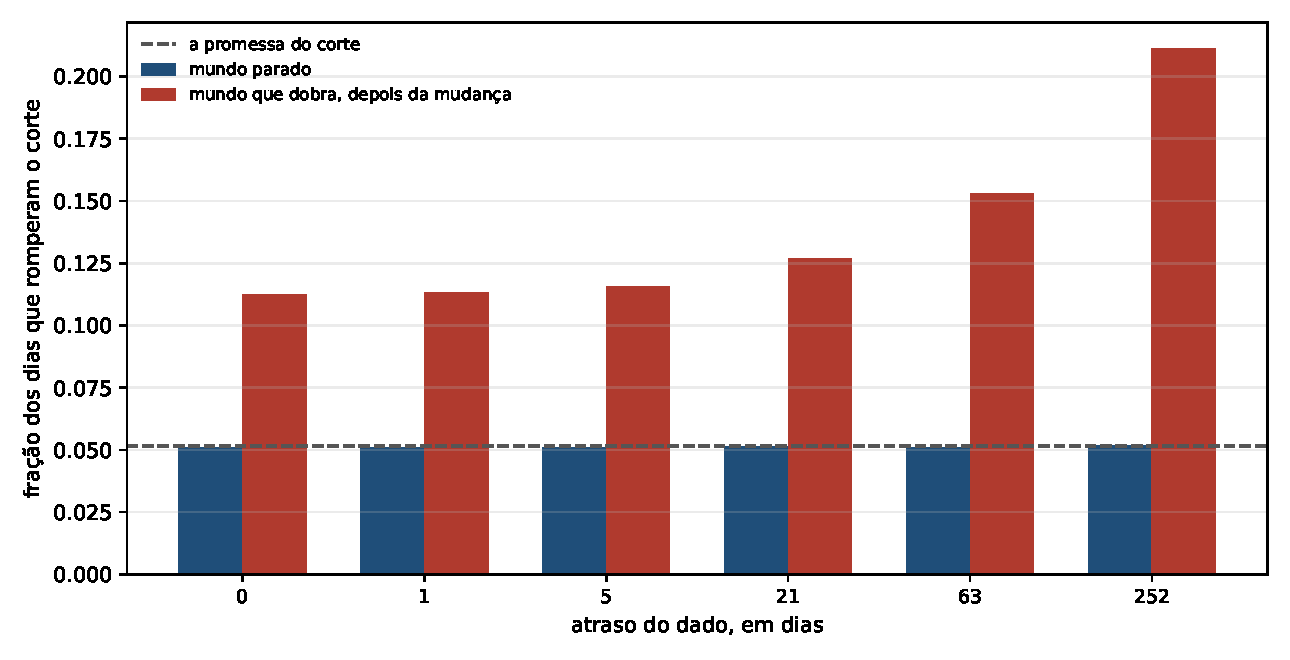
\includegraphics[width=\linewidth]{figuras/E19_o_agora_2.pdf}
  \caption{O mundo parado e o mundo que dobra, por atraso --- o parado medido na série inteira e o
    que dobra na janela que segue a mudança. A barra azul é o controle: ela fica na promessa em
    todos os atrasos.}
  \label{fig:atraso-por-mundo}
\end{figure}

\section{O agora é uma janela}

Com este capítulo o enquadramento fecha, e ele fecha numa imagem só. No instante da decisão --- chamado $t$ ---, o que
um sistema tem é um \textbf{retângulo}: o eixo do tempo vai de $t$ menos o atraso menos a memória até
$t$ menos o atraso. Com atraso nenhum a borda da direita encosta no agora, e o retângulo é o do
capítulo da memória.

A borda da direita é o atraso, medido aqui. A borda da esquerda é a memória, medida duas vezes neste
livro: pela taxa de esquecimento, que diz quanto do passado ainda pesa, e pelo horizonte de
recuperação, que diz até onde o passado apagado volta. E o capítulo anterior mostrou que o próprio
eixo --- onde a série começa e termina --- também é uma escolha.

Nenhuma das três bordas é um fato sobre o mundo. As três são declarações do instrumento, e as três
foram medidas: a individuação, o atraso e a memória. O que sobra depois delas é a pergunta da raiz,
agora com preço conhecido.

\section{O que fica}

Fica a regra do andar do enquadramento, e ela vale para qualquer medição futura: \textbf{declarar as três
bordas}. Onde a série começa e termina, quanto tempo o dado tem, e quanto passado ainda conta.
Nenhuma delas é neutra, e as três foram medidas separadamente neste livro --- com a mesma conclusão
nos três casos, que é a conclusão do livro inteiro: a borda escolhida não é a resposta, e o que
aparece quando ela se mexe é o que ela escondia.

A espiral tem um movimento só por fazer, e ele reaproveita tudo o que já está construído: refazer a pergunta da
raiz. O corte, o orçamento do alarme, a
geometria, a dependência, o esquecimento e o enquadramento já foram medidos; falta lê-los juntos e
responder, com número, o que se pode garantir, medir e otimizar quando o mundo não para de mudar.
